\documentclass[12pt]{article}
\usepackage{hyperref,amsmath,amsfonts,amssymb,fullpage,color,graphicx,tikz}
\usetikzlibrary{decorations.pathmorphing,patterns}
\newcommand{\be}{\begin{equation}}
\newcommand{\ee}{\end{equation}}
\newcommand{\bh}{\bar{h}}
\usepackage{enumitem}
\newcounter{quesno}
\newcommand{\ques}[1]{\vspace{2em}\stepcounter{quesno}
\noindent{\bf Question \thequesno.} \emph{(#1 points)\\}
}

\begin{document}

\begin{center}
{\bf\Large General Relativity -- Final Examination Solutions}

\vspace{1em}
{\bf Solutions and Detailed Derivations}
\end{center}

\vspace{1em}
\hrule
\vspace{1em}

% -------------------------------------------------------------
% QUESTION 1
% -------------------------------------------------------------
\ques{2}
\noindent{\bf Statement:}\\
The components of the Riemann tensor in some coordinates are $R^\mu{}_{\nu\rho\sigma}$.
Write down how they transform under a change of coordinates.
Define the Ricci tensor by $R_{\mu\nu} = R^\rho{}_{\mu\rho\nu}$, and show explicitly that this transforms as a tensor under change of coordinates.

\vspace{1em}
\noindent{\bf Solution:}\\
Under a general coordinate transformation from $x^\mu$ to $x'^\mu$, a $(1,3)$ tensor transforms with one Jacobian matrix factor $\frac{\partial x'^\mu}{\partial x^\alpha}$ for the upper index and three inverse Jacobian matrix factors for each of the lower indices:
\begin{equation}
R'^\mu{}_{\nu\rho\sigma}(x') = \frac{\partial x'^\mu}{\partial x^\alpha} \frac{\partial x^\beta}{\partial x'^\nu} \frac{\partial x^\gamma}{\partial x'^\rho} \frac{\partial x^\delta}{\partial x'^\sigma} R^\alpha{}_{\beta\gamma\delta}(x).
\label{eq:riemann_transform}
\end{equation}

Now, the Ricci tensor is defined by contracting the first upper index with the second lower index (the third slot of the tensor):
\begin{equation}
R_{\mu\nu} = R^\rho{}_{\mu\rho\nu}.
\end{equation}
Applying the transformation law \eqref{eq:riemann_transform} to the primed coordinates:
\begin{equation}
R'_{\mu\nu}(x') = R'^\rho{}_{\mu\rho\nu}(x') = \frac{\partial x'^\rho}{\partial x^\alpha} \frac{\partial x^\beta}{\partial x'^\mu} \frac{\partial x^\gamma}{\partial x'^\rho} \frac{\partial x^\delta}{\partial x'^\nu} R^\alpha{}_{\beta\gamma\delta}(x).
\end{equation}
We can group the two transformation matrices involving the contracted index $x'^\rho$:
\begin{equation}
\frac{\partial x'^\rho}{\partial x^\alpha} \frac{\partial x^\gamma}{\partial x'^\rho} = \frac{\partial x^\gamma}{\partial x'^\rho} \frac{\partial x'^\rho}{\partial x^\alpha} = \frac{\partial x^\gamma}{\partial x^\alpha} = \delta^\gamma_\alpha,
\end{equation}
by the chain rule of multivariable calculus. Substituting this back into the transformation expression:
\begin{align}
R'_{\mu\nu}(x') &= \delta^\gamma_\alpha \frac{\partial x^\beta}{\partial x'^\mu} \frac{\partial x^\delta}{\partial x'^\nu} R^\alpha{}_{\beta\gamma\delta}(x) \nonumber \\
&= \frac{\partial x^\beta}{\partial x'^\mu} \frac{\partial x^\delta}{\partial x'^\nu} R^\alpha{}_{\beta\alpha\delta}(x).
\end{align}
By the definition of the Ricci tensor in the unprimed coordinate frame, $R^\alpha{}_{\beta\alpha\delta}(x) = R_{\beta\delta}(x)$. Therefore, relabeling dummy indices if desired:
\begin{equation}
R'_{\mu\nu}(x') = \frac{\partial x^\beta}{\partial x'^\mu} \frac{\partial x^\delta}{\partial x'^\nu} R_{\beta\delta}(x).
\end{equation}
This is precisely the transformation law for a $(0,2)$ tensor. Hence, the Ricci tensor $R_{\mu\nu}$ transforms as a tensor under coordinate changes.

\vspace{1.5em}
\hrule

% -------------------------------------------------------------
% QUESTION 2
% -------------------------------------------------------------
\ques{3}
\noindent{\bf Statement:}\\
Consider a manifold on which we have both a metric, $g_{\mu\nu}$, and a totally antisymmetric $(0,3)$ tensor, $H_{\mu\nu\rho} = H_{[\mu\nu\rho]}$.
We can define a connection with components $\hat\Gamma_{\mu\nu}{}^\rho$ by:
\be
\hat \Gamma_{\mu\nu}{}^\rho = \Gamma_{\mu\nu}{}^\rho + \frac{1}{12} g^{\rho \sigma} H_{\mu\nu\sigma}
\label{stringconn}
\ee
where $\Gamma_{\mu\nu}{}^\rho$ denotes the components of the usual Levi-Civita connection.

\begin{enumerate}[label=\alph*)]
\item (\emph{2 points}) Is the new connection $\hat\Gamma_{\mu\nu}{}^\rho$ defined in equation \eqref{stringconn} torsion-free? Is it metric compatible? 
\item (\emph{1 point}) Show that the geodesics of the connection $\hat\Gamma_{\mu\nu}{}^\rho$ are the same as the geodesics of the Levi-Civita connection. 
\end{enumerate}

\vspace{1em}
\noindent{\bf Solution:}\\
\begin{enumerate}[label=\alph*)]
\item \textbf{Torsion:}\\
The torsion tensor $T^\rho{}_{\mu\nu}$ of a connection $\hat{\Gamma}_{\mu\nu}{}^\rho$ is defined as the antisymmetric part of the connection in its lower indices:
\begin{equation}
\hat{T}^\rho{}_{\mu\nu} = \hat{\Gamma}_{\mu\nu}{}^\rho - \hat{\Gamma}_{\nu\mu}{}^\rho.
\end{equation}
Since the Levi-Civita connection is torsion-free, $\Gamma_{\mu\nu}{}^\rho = \Gamma_{\nu\mu}{}^\rho$. Substituting \eqref{stringconn}:
\begin{equation}
\hat{T}^\rho{}_{\mu\nu} = \left(\Gamma_{\mu\nu}{}^\rho + \frac{1}{12} g^{\rho\sigma} H_{\mu\nu\sigma}\right) - \left(\Gamma_{\nu\mu}{}^\rho + \frac{1}{12} g^{\rho\sigma} H_{\nu\mu\sigma}\right) = \frac{1}{12} g^{\rho\sigma} \left( H_{\mu\nu\sigma} - H_{\nu\mu\sigma} \right).
\end{equation}
Since $H$ is totally antisymmetric, $H_{\nu\mu\sigma} = - H_{\mu\nu\sigma}$. Therefore:
\begin{equation}
\hat{T}^\rho{}_{\mu\nu} = \frac{1}{12} g^{\rho\sigma} \left( 2 H_{\mu\nu\sigma} \right) = \frac{1}{6} g^{\rho\sigma} H_{\mu\nu\sigma} = \frac{1}{6} H_{\mu\nu}{}^\rho.
\end{equation}
Unless $H_{\mu\nu\rho} \equiv 0$, the torsion tensor is non-zero. Thus, \textbf{the new connection is not torsion-free}.

\vspace{0.8em}
\noindent\textbf{Metric Compatibility:}\\
A connection is metric compatible if the covariant derivative of the metric with respect to this connection vanishes, i.e., $\hat{\nabla}_\lambda g_{\mu\nu} = 0$. 
The covariant derivative acting on a $(0,2)$ tensor is:
\begin{equation}
\hat{\nabla}_\lambda g_{\mu\nu} = \partial_\lambda g_{\mu\nu} - \hat{\Gamma}_{\lambda\mu}{}^\rho g_{\rho\nu} - \hat{\Gamma}_{\lambda\nu}{}^\rho g_{\mu\rho}.
\end{equation}
Using $\hat{\Gamma}_{\lambda\mu}{}^\rho = \Gamma_{\lambda\mu}{}^\rho + \frac{1}{12} g^{\rho\sigma} H_{\lambda\mu\sigma}$, we have:
\begin{align}
\hat{\nabla}_\lambda g_{\mu\nu} &= \left( \partial_\lambda g_{\mu\nu} - \Gamma_{\lambda\mu}{}^\rho g_{\rho\nu} - \Gamma_{\lambda\nu}{}^\rho g_{\mu\rho} \right) - \frac{1}{12} g^{\rho\sigma} H_{\lambda\mu\sigma} g_{\rho\nu} - \frac{1}{12} g^{\rho\sigma} H_{\lambda\nu\sigma} g_{\mu\rho} \nonumber \\
&= \nabla_\lambda g_{\mu\nu} - \frac{1}{12} \delta^\sigma_\nu H_{\lambda\mu\sigma} - \frac{1}{12} \delta^\sigma_\mu H_{\lambda\nu\sigma}.
\end{align}
Because the Levi-Civita connection is metric-compatible, $\nabla_\lambda g_{\mu\nu} = 0$. Thus:
\begin{equation}
\hat{\nabla}_\lambda g_{\mu\nu} = - \frac{1}{12} \left( H_{\lambda\mu\nu} + H_{\lambda\nu\mu} \right).
\end{equation}
Since $H$ is totally antisymmetric, swapping the last two indices gives $H_{\lambda\nu\mu} = - H_{\lambda\mu\nu}$. Therefore:
\begin{equation}
H_{\lambda\mu\nu} + H_{\lambda\nu\mu} = H_{\lambda\mu\nu} - H_{\lambda\mu\nu} = 0.
\end{equation}
Hence,
\begin{equation}
\hat{\nabla}_\lambda g_{\mu\nu} = 0.
\end{equation}
Thus, \textbf{the connection is metric compatible}.

\item \textbf{Geodesics:}\\
The geodesic equation for an affinely parameterised curve $x^\rho(\lambda)$ with tangent vector $u^\mu = \frac{dx^\mu}{d\lambda}$ with respect to the connection $\hat{\Gamma}$ is:
\begin{equation}
\frac{d^2 x^\rho}{d\lambda^2} + \hat{\Gamma}_{\mu\nu}{}^\rho \frac{dx^\mu}{d\lambda} \frac{dx^\nu}{d\lambda} = 0.
\end{equation}
Substituting the definition of $\hat{\Gamma}_{\mu\nu}{}^\rho$:
\begin{equation}
\frac{d^2 x^\rho}{d\lambda^2} + \Gamma_{\mu\nu}{}^\rho \frac{dx^\mu}{d\lambda} \frac{dx^\nu}{d\lambda} + \frac{1}{12} g^{\rho\sigma} H_{\mu\nu\sigma} \frac{dx^\mu}{d\lambda} \frac{dx^\nu}{d\lambda} = 0.
\end{equation}
Notice that the term $\frac{dx^\mu}{d\lambda} \frac{dx^\nu}{d\lambda}$ is completely symmetric under the exchange of indices $\mu \leftrightarrow \nu$, whereas $H_{\mu\nu\sigma}$ is totally antisymmetric, and therefore antisymmetric under $\mu \leftrightarrow \nu$ ($H_{\mu\nu\sigma} = -H_{\nu\mu\sigma}$). 
Contracting a symmetric tensor with an antisymmetric tensor vanishes identically:
\begin{equation}
H_{\mu\nu\sigma} \frac{dx^\mu}{d\lambda} \frac{dx^\nu}{d\lambda} = - H_{\nu\mu\sigma} \frac{dx^\mu}{d\lambda} \frac{dx^\nu}{d\lambda} = - H_{\mu\nu\sigma} \frac{dx^\nu}{d\lambda} \frac{dx^\mu}{d\lambda} = - H_{\mu\nu\sigma} \frac{dx^\mu}{d\lambda} \frac{dx^\nu}{d\lambda} \implies H_{\mu\nu\sigma} \frac{dx^\mu}{d\lambda} \frac{dx^\nu}{d\lambda} = 0.
\end{equation}
Therefore, the geodesic equation reduces to:
\begin{equation}
\frac{d^2 x^\rho}{d\lambda^2} + \Gamma_{\mu\nu}{}^\rho \frac{dx^\mu}{d\lambda} \frac{dx^\nu}{d\lambda} = 0,
\end{equation}
which is precisely the geodesic equation for the Levi-Civita connection $\Gamma_{\mu\nu}{}^\rho$. Hence, the affinely parameterised geodesics of $\hat{\Gamma}$ and $\Gamma$ are identical.
\end{enumerate}

\vspace{1.5em}
\hrule

% -------------------------------------------------------------
% QUESTION 3
% -------------------------------------------------------------
\ques{4}
\noindent{\bf Statement:}\\
The Schwarzschild metric is:
\be
ds^2 = - f(r) dt^2 + f(r)^{-1} dr^2 + r^2 d \theta^2 + r^2 \sin^2 \theta d\phi^2 
\ee
where $f(r) = 1 - \frac{2GM}{r}$. 

\begin{enumerate}[label=\alph*)]
\item (\emph{2 points}) Suppose you are sufficiently interested in physics that you decide to fall into a Schwarzschild black hole to see what happens. 
Your friends and family think this might be unsafe, as they have noticed there are singularities in the Schwarzschild metric. 
Where do these singularities occur, which should you be genuinely concerned about, and why? 
\item (\emph{2 points}) Determine the Schwarzschild metric in the ingoing Eddington-Finkelstein coordinates $(v,r,\theta,\phi)$, where
\be
v = t + r + 2GM \ln\left| \frac{r}{2GM} - 1 \right|
\ee
and explain how this supports your answer to part a). 
\end{enumerate}

\vspace{1em}
\noindent{\bf Solution:}\\
\begin{enumerate}[label=\alph*)]
\item Looking at the Schwarzschild metric components:
\begin{equation}
g_{tt} = - \left(1 - \frac{2GM}{r}\right), \quad g_{rr} = \left(1 - \frac{2GM}{r}\right)^{-1},
\end{equation}
metric components exhibit singularities at two locations:
\begin{enumerate}[label=(\roman*)]
\item At $r = 2GM$, where $g_{tt} = 0$ and $g_{rr} \to \infty$.
\item At $r = 0$, where $g_{tt} \to \infty$, $g_{rr} \to 0$, and the angular components $g_{\theta\theta}=0, g_{\phi\phi}=0$.
\end{enumerate}

To determine which of these represent genuine physical singularities (where spacetime curvature diverges and tidal forces become infinite) versus coordinate artifacts (due to a breakdown of the chosen coordinate chart), we compute coordinate-invariant quantities, such as curvature invariants. 
For Schwarzschild spacetime, the Ricci scalar and Ricci tensor vanish in vacuum ($R = 0, R_{\mu\nu} = 0$), so the leading invariant is the Kretschmann scalar:
\begin{equation}
K = R^{\alpha\beta\gamma\delta} R_{\alpha\beta\gamma\delta} = \frac{48 G^2 M^2}{r^6}.
\end{equation}
Evaluating this scalar at both locations:
\begin{itemize}
\item At $r = 2GM$:
\begin{equation}
K\Big|_{r=2GM} = \frac{48 G^2 M^2}{(2GM)^6} = \frac{3}{4 G^4 M^4} < \infty.
\end{equation}
The Kretschmann scalar (as well as all other curvature invariants) is completely smooth, finite, and non-singular at $r = 2GM$. This indicates that $r = 2GM$ is merely a \textbf{coordinate singularity} (the event horizon). An infalling observer crosses $r = 2GM$ in finite proper time without experiencing infinite tidal forces (for a supermassive black hole, tidal forces at the horizon can even be negligible).
\item At $r = 0$:
\begin{equation}
\lim_{r\to 0} K = \lim_{r\to 0} \frac{48 G^2 M^2}{r^6} = \infty.
\end{equation}
The curvature invariant diverges to infinity. This is a \textbf{true physical (gravitational) singularity}. 
\end{itemize}
Therefore, you should only be genuinely concerned about the physical singularity at \textbf{$r = 0$}, where infinite spacetime curvature produces infinite tidal forces that will inevitably destroy (spaghettify) any physical observer. The singularity at $r = 2GM$ is an artifact of Schwarzschild coordinates and does not pose any danger from infinite curvature.

\item We introduce the ingoing Eddington-Finkelstein coordinate $v$:
\begin{equation}
v = t + r^*, \quad \text{where } r^* = r + 2GM \ln\left|\frac{r}{2GM} - 1\right|.
\end{equation}
Differentiating $r^*$:
\begin{equation}
dr^* = dr + 2GM \frac{1}{\frac{r}{2GM} - 1} \frac{dr}{2GM} = dr + \frac{dr}{\frac{r}{2GM} - 1} = \left( 1 + \frac{2GM}{r - 2GM} \right) dr = \frac{r}{r - 2GM} dr = f(r)^{-1} dr.
\end{equation}
Therefore, taking the differential of $v$:
\begin{equation}
dv = dt + dr^* = dt + f(r)^{-1} dr \implies dt = dv - f(r)^{-1} dr.
\end{equation}
Now, substitute $dt$ into the Schwarzschild line element:
\begin{align}
ds^2 &= - f(r) dt^2 + f(r)^{-1} dr^2 + r^2 d\Omega^2 \nonumber \\
&= - f(r) \left( dv - f(r)^{-1} dr \right)^2 + f(r)^{-1} dr^2 + r^2 d\Omega^2 \nonumber \\
&= - f(r) \left( dv^2 - 2 f(r)^{-1} dv dr + f(r)^{-2} dr^2 \right) + f(r)^{-1} dr^2 + r^2 d\Omega^2 \nonumber \\
&= - f(r) dv^2 + 2 dv dr - f(r)^{-1} dr^2 + f(r)^{-1} dr^2 + r^2 d\Omega^2 \nonumber \\
&= - f(r) dv^2 + 2 dv dr + r^2 \left( d\theta^2 + \sin^2\theta d\phi^2 \right).
\end{align}
With $f(r) = 1 - \frac{2GM}{r}$, the metric in $(v,r,\theta,\phi)$ coordinates is:
\begin{equation}
ds^2 = - \left( 1 - \frac{2GM}{r} \right) dv^2 + 2 dv dr + r^2 \left( d\theta^2 + \sin^2\theta d\phi^2 \right).
\end{equation}

\noindent\textbf{Explanation and connection to part a):}\\
In these coordinates, the metric components are:
\begin{equation}
g_{\mu\nu} = \begin{pmatrix}
-(1 - 2GM/r) & 1 & 0 & 0 \\
1 & 0 & 0 & 0 \\
0 & 0 & r^2 & 0 \\
0 & 0 & 0 & r^2\sin^2\theta
\end{pmatrix}.
\end{equation}
The determinant of this metric is:
\begin{equation}
\det(g) = \left[ -(1 - 2GM/r) \cdot 0 - 1 \cdot 1 \right] \cdot r^4 \sin^2\theta = - r^4 \sin^2\theta.
\end{equation}
Notice that:
\begin{itemize}
\item Every component of the metric $g_{\mu\nu}$ and its inverse $g^{\mu\nu}$ is completely smooth, well-behaved, and non-singular at $r = 2GM$. The determinant is $\det(g) = - (2GM)^4 \sin^2\theta \neq 0$ at $r = 2GM$.
\item Radial ingoing null geodesics satisfy $dv = 0$, along which $v = \text{const.}$, and as $r$ decreases, light and freely falling observers smoothly pass across $r = 2GM$ into $r < 2GM$ without encounter of infinite values.
\item On the other hand, at $r = 0$, the metric component $g_{vv} \to \infty$ and $\det(g) = 0$, confirming that $r=0$ remains singular.
\end{itemize}
This explicitly demonstrates that the apparent divergence at $r = 2GM$ in Schwarzschild coordinates was merely a coordinate singularity due to a failing coordinate chart, whereas the geometry itself is smooth across $r = 2GM$.
\end{enumerate}

\vspace{1.5em}
\hrule

% -------------------------------------------------------------
% QUESTION 4
% -------------------------------------------------------------
\ques{5}
\noindent{\bf Statement:}\\
The metric of de Sitter is:
\be
ds^2 =- dt^2 +  L^2  \cosh^2 (t/L) \left( d\chi^2 + \sin^2 \chi \left( d\theta^2 + \sin^2\theta d\phi^2 \right)\right)  \,.
\label{dsmetric} 
\ee
where $t \in (-\infty, \infty)$, $\chi \in (0,\pi)$ and $(\theta,\phi)$ are the usual coordinates on a two-sphere (and together $\chi, \theta,\phi$ parametrise a three-sphere).

\begin{enumerate}[label=\alph*)]
\item (\emph{2 points}) Explain why this metric is a candidate cosmological solution that could describe our universe. What is the scale factor?  
\item (\emph{1 point}) Explain why two metrics that are related by $g_{\mu\nu} = \Omega^2 \bar g_{\mu\nu}$, can be said to have the same causal structure. 
\item (\emph{2 points}) For de Sitter, make the coordinate transformation
\be
\cosh \frac{t}{L} = \frac{1}{\cos \eta} \,,
\ee
and draw the Penrose diagram. 
\end{enumerate}

\vspace{1em}
\noindent{\bf Solution:}\\
\begin{enumerate}[label=\alph*)]
\item The general Friedmann-Lema\^itre-Robertson-Walker (FLRW) metric describing a homogeneous and isotropic universe is given by:
\begin{equation}
ds^2 = - dt^2 + a(t)^2 d\Sigma_k^2,
\end{equation}
where $t$ is cosmic (proper) time, $a(t)$ is the cosmological scale factor, and $d\Sigma_k^2$ is the metric of a maximally symmetric 3-space of constant curvature $k \in \{+1, 0, -1\}$. For a closed 3-sphere ($k=+1$), the metric is:
\begin{equation}
d\Sigma_{k=+1}^2 = d\chi^2 + \sin^2\chi (d\theta^2 + \sin^2\theta d\phi^2).
\end{equation}
Comparing the given de Sitter metric \eqref{dsmetric} with the FLRW metric:
\begin{equation}
ds^2 = - dt^2 + \left[ L \cosh(t/L) \right]^2 d\Sigma_{k=+1}^2,
\end{equation}
we see that de Sitter spacetime is an exact closed ($k=+1$) FLRW solution with scale factor:
\begin{equation}
a(t) = L \cosh(t/L).
\end{equation}
\textbf{Why it is a candidate cosmological solution:}\\
\begin{enumerate}[label=(\roman*)]
\item It is maximally symmetric, hence strictly homogeneous and isotropic, in accordance with the Cosmological Principle observed on cosmological scales.
\item It solves Einstein's equations in the presence of a positive cosmological constant $\Lambda = 3/L^2$ (or dark energy):
\begin{equation}
G_{\mu\nu} + \Lambda g_{\mu\nu} = 0 \iff R_{\mu\nu} = \frac{3}{L^2} g_{\mu\nu}.
\end{equation}
\item For late times $t \gg L$, $\cosh(t/L) \approx \frac{1}{2} e^{t/L}$, yielding an exponentially expanding universe $a(t) \propto e^{H t}$ with Hubble parameter $H = 1/L$. Observational cosmology indicates that our current universe is accelerated and dominated by dark energy ($\sim 70\%$ dark energy density), meaning our universe is asymptotically approaching a de Sitter phase. It is also the paradigm for early-universe cosmic inflation.
\end{enumerate}

\item Two metrics $g_{\mu\nu}$ and $\bar{g}_{\mu\nu}$ related by a conformal transformation $g_{\mu\nu} = \Omega^2(x) \bar{g}_{\mu\nu}$ (where $\Omega(x) > 0$ is a smooth, strictly positive non-vanishing scalar factor) have the exact same causal structure because the character of any tangent vector $v^\mu$ is preserved:
\begin{equation}
g_{\mu\nu} v^\mu v^\nu = \Omega^2(x) \left( \bar{g}_{\mu\nu} v^\mu v^\nu \right).
\end{equation}
Since $\Omega^2(x) > 0$:
\begin{align}
g_{\mu\nu} v^\mu v^\nu < 0 &\iff \bar{g}_{\mu\nu} v^\mu v^\nu < 0 \quad (\text{timelike}), \\
g_{\mu\nu} v^\mu v^\nu = 0 &\iff \bar{g}_{\mu\nu} v^\mu v^\nu = 0 \quad (\text{null / lightlike}), \\
g_{\mu\nu} v^\mu v^\nu > 0 &\iff \bar{g}_{\mu\nu} v^\mu v^\nu > 0 \quad (\text{spacelike}).
\end{align}
In particular, light cones (null surfaces) are identical at every spacetime point: $ds^2 = 0 \iff d\bar{s}^2 = 0$. Consequently, the trajectories of light rays and the causal relationships between any two events (whether an event can be influenced by, influence, or be causally disconnected from another) are completely identical in both spacetimes.

\item \textbf{Coordinate Transformation and Conformal Metric:}\\
We are given the relation:
\begin{equation}
\cosh\frac{t}{L} = \frac{1}{\cos\eta}.
\end{equation}
Since $t \in (-\infty, \infty)$, we have $\cosh(t/L) \in [1, \infty)$. To match this range with $\cos\eta \in (0, 1]$, the conformal time $\eta$ must lie in the range:
\begin{equation}
\eta \in \left(-\frac{\pi}{2}, \frac{\pi}{2}\right),
\end{equation}
with $t \to -\infty \iff \eta \to -\frac{\pi}{2}$, $t = 0 \iff \eta = 0$, and $t \to +\infty \iff \eta \to \frac{\pi}{2}$.

Differentiating both sides with respect to $\eta$:
\begin{equation}
\frac{d}{dt}\left(\cosh\frac{t}{L}\right) dt = \frac{d}{d\eta}\left(\frac{1}{\cos\eta}\right) d\eta \implies \frac{1}{L} \sinh\frac{t}{L} dt = \frac{\sin\eta}{\cos^2\eta} d\eta.
\end{equation}
Using the hyperbolic identity $\sinh^2(t/L) = \cosh^2(t/L) - 1 = \frac{1}{\cos^2\eta} - 1 = \frac{1 - \cos^2\eta}{\cos^2\eta} = \frac{\sin^2\eta}{\cos^2\eta} = \tan^2\eta$:
\begin{equation}
\sinh\frac{t}{L} = \tan\eta = \frac{\sin\eta}{\cos\eta}.
\end{equation}
Thus,
\begin{equation}
\frac{1}{L} \left(\frac{\sin\eta}{\cos\eta}\right) dt = \frac{\sin\eta}{\cos^2\eta} d\eta \implies dt = \frac{L}{\cos\eta} d\eta.
\end{equation}
Now substituting $dt$ and $\cosh(t/L) = \frac{1}{\cos\eta}$ into the de Sitter metric \eqref{dsmetric}:
\begin{align}
ds^2 &= - \left(\frac{L}{\cos\eta} d\eta\right)^2 + L^2 \left(\frac{1}{\cos\eta}\right)^2 \left[ d\chi^2 + \sin^2\chi (d\theta^2 + \sin^2\theta d\phi^2) \right] \nonumber \\
&= \frac{L^2}{\cos^2\eta} \left[ - d\eta^2 + d\chi^2 + \sin^2\chi (d\theta^2 + \sin^2\theta d\phi^2) \right].
\end{align}
This is conformally equivalent to the Einstein static universe:
\begin{equation}
ds^2 = \Omega(\eta)^2 d\bar{s}^2, \quad \text{where } \Omega(\eta) = \frac{L}{\cos\eta}, \quad d\bar{s}^2 = - d\eta^2 + d\chi^2 + \sin^2\chi d\Omega_2^2.
\end{equation}

\vspace{0.8em}
\noindent\textbf{Penrose Diagram:}\\
In the conformal metric $d\bar{s}^2$, null geodesics in the $(\eta, \chi)$ plane are straight lines inclined at $45^\circ$, satisfying:
\begin{equation}
d\eta = \pm d\chi.
\end{equation}
The coordinates span:
\begin{equation}
\chi \in [0, \pi], \quad \eta \in \left[-\frac{\pi}{2}, \frac{\pi}{2}\right].
\end{equation}
This defines a square (or rectangle of aspect ratio $1:1$) in the $(\chi, \eta)$ plane:
\begin{itemize}
\item The bottom boundary at $\eta = -\pi/2$ corresponds to past timelike/null infinity $\mathcal{I}^-$, which is a spacelike 3-sphere ($t \to -\infty$).
\item The top boundary at $\eta = +\pi/2$ corresponds to future timelike/null infinity $\mathcal{I}^+$, which is a spacelike 3-sphere ($t \to +\infty$).
\item The left edge $\chi = 0$ is the North Pole of the 3-sphere (a coordinate origin / regular axis).
\item The right edge $\chi = \pi$ is the South Pole of the 3-sphere (the antipodal regular axis).
\end{itemize}

\begin{center}
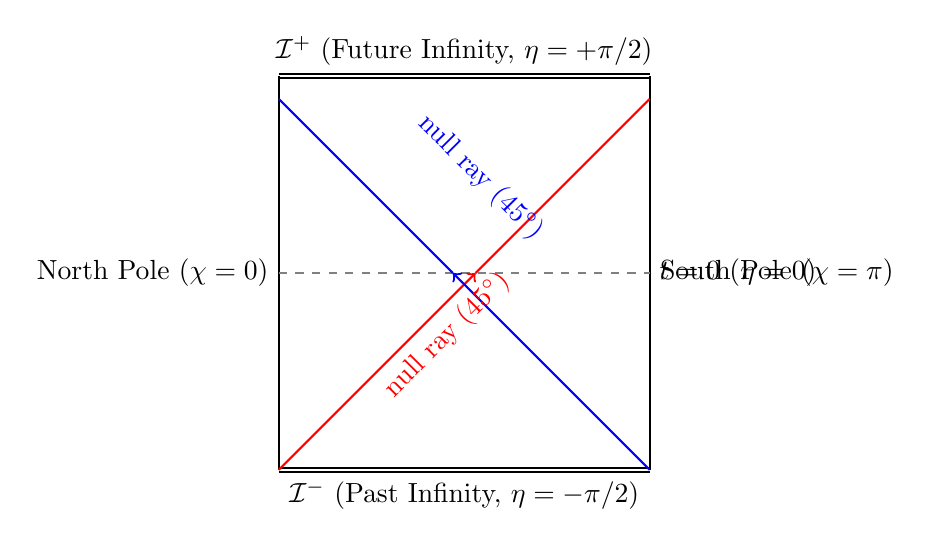
\begin{tikzpicture}[scale=2.5]
    % Boundaries
    \draw[thick, double] (0, 1) -- (3.14159/2*1.2, 1) node[midway, above] {$\mathcal{I}^+$ (Future Infinity, $\eta = +\pi/2$)};
    \draw[thick, double] (0, -1) -- (3.14159/2*1.2, -1) node[midway, below] {$\mathcal{I}^-$ (Past Infinity, $\eta = -\pi/2$)};
    \draw[thick] (0, -1) -- (0, 1) node[midway, left] {North Pole ($\chi = 0$)};
    \draw[thick] (3.14159/2*1.2, -1) -- (3.14159/2*1.2, 1) node[midway, right] {South Pole ($\chi = \pi$)};
    
    % Mid line
    \draw[dashed, gray] (0,0) -- (3.14159/2*1.2, 0) node[right, black] {$t=0$ ($\eta = 0$)};
    
    % Light rays (45 degrees)
    \draw[thick, red, ->] (0, -1) -- (1, 0);
    \draw[thick, red] (1, 0) -- (1.885, 0.885);
    \draw[thick, blue, ->] (1.885, -1) -- (0.885, 0);
    \draw[thick, blue] (0.885, 0) -- (0, 0.885);
    
    % Labels
    \node at (0.94, -0.4) [rotate=45, red, above] {null ray ($45^\circ$)};
    \node at (0.94, 0.4) [rotate=-45, blue, above] {null ray ($45^\circ$)};
\end{tikzpicture}
\end{center}
Both $\mathcal{I}^+$ and $\mathcal{I}^-$ are spacelike surfaces, reflecting the cosmological expansion of de Sitter space.
\end{enumerate}

\vspace{1.5em}
\hrule

% -------------------------------------------------------------
% QUESTION 5
% -------------------------------------------------------------
\ques{6}
\noindent{\bf Statement:}\\
The linearised Einstein equation is
\be
- \frac{1}{2} \partial^\rho\partial_\rho \bh_{\mu\nu} + \partial^\rho \partial_{(\mu} \bh_{\nu)\rho}
- \frac{1}{2} \eta_{\mu\nu} \partial^\rho \partial^\sigma \bh_{\rho\sigma} = 8 \pi G T_{\mu\nu} \,,
\ee
when written in terms of $\bh_{\mu\nu} = h_{\mu\nu} - \frac{1}{2} h \eta_{\mu\nu}$. 

\begin{enumerate}[label=\alph*)]
\item (\emph{1 point}) By making an appropriate gauge choice, explain why the linearised Einstein equation leads to \emph{gravitational waves}.
\item (\emph{2 point}) Consider an experiment involving two freely falling test particles, arranged so that one is at spatial position $x^i = (0,0,0)$ and the other at spatial position $x^i=(L_x,0,0)$.
Suppose a gravitational wave travelling along the $z$-axis passes through the laboratory, corresponding to the following metric perturbation:
\be
h_{\mu\nu} = \begin{pmatrix}
0 & 0 & 0 & 0 \\
0 & h_{+}(t-z) & 0 & 0 \\
0 & 0 & - h_{+}(t-z) & 0 \\
0 & 0 & 0 & 0
\end{pmatrix} \,.
\ee
Show that the proper distance between the test particles is given by: 
\be
\Delta s \approx L_x \left( 1 + \frac{1}{2} h_{+}(t) \right) \,.
\ee
If a third test particle is introduced at $x^i=(0,L_y,0)$ show that the proper distance between it and the particle at the origin is
\be
\Delta s \approx L_y \left( 1 - \frac{1}{2} h_{+}(t) \right) \,.
\ee
\item (\emph{3 points}) Consider a binary system consisting of two massive bodies in a circular orbit, which are emitting gravitational waves.
Explain \emph{qualitatively} what happens to the system, and sketch the corresponding gravitational wave signal which would be observed by a detector such as LIGO.
You should mention the following terms: \emph{inspiral}, \emph{merger}, \emph{ringdown}, explain how the interferometer detects a wave such as that described in part b), and connect the features of the signal to the physics of the binary pair. 
\end{enumerate}

\vspace{1em}
\noindent{\bf Solution:}\\
\begin{enumerate}[label=\alph*)]
\item Under an infinitesimal coordinate transformation (gauge transformation) $x^\mu \to x^\mu - \xi^\mu$, the trace-reversed perturbation transforms as:
\begin{equation}
\bar{h}_{\mu\nu} \to \bar{h}_{\mu\nu} + \partial_\mu \xi_\nu + \partial_\nu \xi_\mu - \eta_{\mu\nu} \partial_\rho \xi^\rho.
\end{equation}
This allows us to choose the \textbf{Lorenz gauge} (also known as the de Donder, Hilbert, or harmonic gauge):
\begin{equation}
\partial^\mu \bar{h}_{\mu\nu} = 0.
\end{equation}
Substituting this condition into the linearized Einstein equation, the second and third terms vanish identically:
\begin{equation}
\partial^\rho \partial_{(\mu} \bar{h}_{\nu)\rho} = 0, \quad \partial^\rho \partial^\sigma \bar{h}_{\rho\sigma} = 0.
\end{equation}
The linearized Einstein equation then dramatically simplifies to:
\begin{equation}
- \frac{1}{2} \Box \bar{h}_{\mu\nu} = 8\pi G T_{\mu\nu} \implies \Box \bar{h}_{\mu\nu} = - 16\pi G T_{\mu\nu},
\end{equation}
where $\Box = \partial^\rho \partial_\rho = -\frac{\partial^2}{\partial t^2} + \nabla^2$ is the flat-space d'Alembertian wave operator.

In vacuum (outside of sources, $T_{\mu\nu} = 0$), this equation becomes:
\begin{equation}
\Box \bar{h}_{\mu\nu} = \left(-\frac{1}{c^2}\frac{\partial^2}{\partial t^2} + \nabla^2\right) \bar{h}_{\mu\nu} = 0.
\end{equation}
This is the standard, relativistic three-dimensional \textbf{wave equation}. Its solutions represent disturbances in the spacetime metric that propagate through vacuum at the speed of light ($c=1$). These propagating metric fluctuations are precisely \textbf{gravitational waves}.

\item In the transverse-traceless (TT) gauge, the coordinates are attached to freely falling particles; that is, particles initially at rest in this frame have four-velocity $u^\mu = (1, 0, 0, 0)$ and the geodesic equation yields $\frac{du^\mu}{d\tau} = - \Gamma^\mu_{00} = 0$ because $\Gamma^\mu_{00} = \frac{1}{2}\eta^{\mu\lambda}(2\partial_0 h_{\lambda 0} - \partial_\lambda h_{00}) = 0$ as $h_{0\mu} = 0$. Hence, the coordinate positions of freely falling test particles remain constant at all times.

The laboratory is situated in the $z=0$ plane, so for both particles $z=0$, giving $h_+(t-z) = h_+(t)$.
\begin{itemize}
\item \textbf{Proper distance along the $x$-axis:}\\
Consider the particle at the origin $(0,0,0)$ and the particle at $(L_x, 0, 0)$ at a fixed coordinate time $t$ ($dt = 0, dy = 0, dz = 0$). 
The spacetime line element along the $x$-axis is:
\begin{equation}
ds^2 = g_{xx} dx^2 = (\eta_{xx} + h_{xx}) dx^2 = (1 + h_+(t)) dx^2.
\end{equation}
The proper spatial distance $\Delta s$ between the origin $x=0$ and $x=L_x$ at time $t$ is obtained by integrating $\sqrt{ds^2}$:
\begin{equation}
\Delta s = \int_0^{L_x} \sqrt{1 + h_+(t)} \, dx = \sqrt{1 + h_+(t)} \int_0^{L_x} dx = L_x \sqrt{1 + h_+(t)}.
\end{equation}
Since linear perturbation theory assumes $|h_+| \ll 1$, we use the Taylor expansion $(1+\epsilon)^{1/2} \approx 1 + \frac{1}{2}\epsilon$:
\begin{equation}
\Delta s \approx L_x \left( 1 + \frac{1}{2} h_+(t) \right).
\end{equation}

\item \textbf{Proper distance along the $y$-axis:}\\
For the third test particle at $(0, L_y, 0)$, we consider the spatial path along the $y$-axis from $y=0$ to $y=L_y$ at fixed $t, x=0, z=0$:
\begin{equation}
ds^2 = g_{yy} dy^2 = (\eta_{yy} + h_{yy}) dy^2 = (1 - h_+(t)) dy^2.
\end{equation}
Integrating to obtain the proper distance:
\begin{equation}
\Delta s = \int_0^{L_y} \sqrt{1 - h_+(t)} \, dy = L_y \sqrt{1 - h_+(t)}.
\end{equation}
Expanding to first order for $|h_+| \ll 1$:
\begin{equation}
\Delta s \approx L_y \left( 1 - \frac{1}{2} h_+(t) \right).
\end{equation}
\end{itemize}

\item \textbf{Binary Coalescence and Gravitational Wave Signal:}

\vspace{0.5em}
\noindent\textbf{1. Qualitative Evolution and Physics of the Binary System:}
Consider two compact massive bodies (such as neutron stars or black holes) in an initial circular orbit:
\begin{itemize}
\item \textbf{Inspiral:} 
As the bodies orbit each other, the time-dependent mass quadrupole moment of the binary produces quadrupole gravitational radiation, continuously carrying away energy and angular momentum from the system. 
According to Kepler's third law, losing orbital energy causes the orbital separation $R$ to shrink ($\dot{R} < 0$). 
As $R$ decreases, the orbital frequency $\Omega = \sqrt{G M_{\text{tot}}/R^3}$ increases, which in turn increases the gravitational wave frequency $f_{\text{GW}} = 2 f_{\text{orb}} = \Omega / \pi$. 
The rate of energy loss also scales strongly with frequency ($\frac{dE}{dt} \propto \Omega^{10/3}$), causing the orbital decay to accelerate. Consequently, both the frequency and amplitude of the gravitational wave increase simultaneously over time. This characteristic signal is known as a \textbf{``chirp''}.

\item \textbf{Merger:} 
Eventually, the two bodies reach the Innermost Stable Circular Orbit (ISCO). Beyond this point, stable circular orbits no longer exist, and the bodies plunge toward each other at relativistic speeds (a significant fraction of the speed of light) and coalesce into a single, highly deformed, highly perturbed remnant black hole. The gravitational wave amplitude and frequency reach their global maximum during this stage.

\item \textbf{Ringdown:} 
The newly formed black hole sheds its asymmetries and perturbations by emitting gravitational radiation governed by its characteristic damped \textbf{quasi-normal modes} (QNMs). The signal during this phase is a rapidly decaying sinusoid:
\begin{equation}
h(t) \sim e^{-t/\tau} \cos(\omega_{\text{QNM}} t + \phi_0).
\end{equation}
According to the no-hair theorem, the ringdown quickly settles into a stationary Kerr black hole characterized entirely by its final mass $M_f$ and spin $a_f$.
\end{itemize}

\vspace{0.8em}
\noindent\textbf{2. Detection by an Interferometer (LIGO):}
A laser interferometer such as LIGO consists of two orthogonal arms of length $L_x = L_y = L$ (along the $x$ and $y$ axes). 
As derived in part b), a passing $+$-polarised gravitational wave travelling along the $z$-axis induces differential arm length variations:
\begin{equation}
\Delta L_x(t) \approx \frac{1}{2} L \, h_+(t), \quad \Delta L_y(t) \approx - \frac{1}{2} L \, h_+(t).
\end{equation}
The differential arm length change is therefore:
\begin{equation}
\delta L(t) = \Delta L_x(t) - \Delta L_y(t) \approx L \, h_+(t).
\end{equation}
This differential displacement creates a time-dependent phase shift $\Delta\Phi(t) = \frac{4\pi}{\lambda_L} \delta L(t) = \frac{4\pi L}{\lambda_L} h_+(t)$ between the laser beams returning from the two arms, which produce constructive/destructive interference at the photodetector. Measuring this interference fringe shift enables LIGO to measure strains $h \sim 10^{-21}$ with extraordinary precision.

\vspace{0.8em}
\noindent\textbf{3. Sketch of the Gravitational Wave Signal:}

\begin{center}
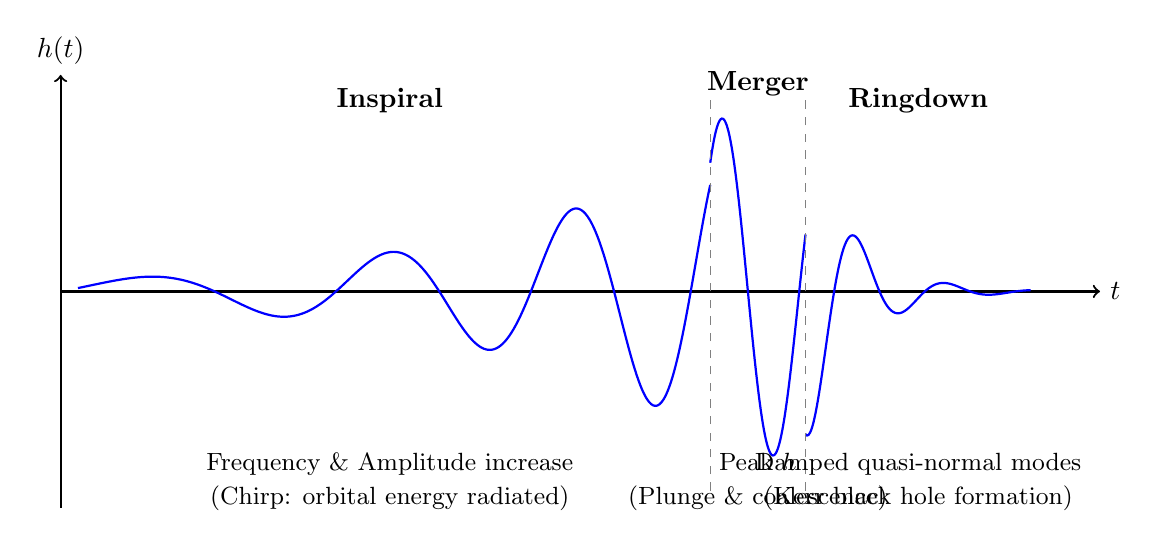
\begin{tikzpicture}[scale=1.1]
    % Axes
    \draw[->, thick] (0,0) -- (12,0) node[right] {$t$};
    \draw[->, thick] (0,-2.5) -- (0,2.5) node[above] {$h(t)$};
    
    % Waveform
    % Inspiral: increasing amplitude and frequency
    \draw[thick, blue, domain=0.2:7.5, samples=300, smooth] 
        plot (\x, {0.12 * exp(0.35*\x) * sin(deg(1.5*\x + 0.15*\x^2))});
        
    % Merger: peak amplitude and highest frequency
    \draw[thick, blue, domain=7.5:8.6, samples=100, smooth] 
        plot (\x, { (2.0 - 0.2*(\x-7.5)^2) * sin(deg(1.5*\x + 0.15*7.5^2 + 3.8*(\x-7.5))) });
        
    % Ringdown: exponentially decaying sinusoid
    \draw[thick, blue, domain=8.6:11.2, samples=150, smooth] 
        plot (\x, { 1.8 * exp(-1.8*(\x-8.6)) * sin(deg(42 + 6.0*(\x-8.6))) });

    % Phase divisions
    \draw[dashed, gray] (7.5,-2.3) -- (7.5,2.3);
    \draw[dashed, gray] (8.6,-2.3) -- (8.6,2.3);
    
    % Phase labels
    \node at (3.8, 2.2) {\bf Inspiral};
    \node at (3.8, -2.2) [align=center] {\small Frequency \& Amplitude increase\\ \small (Chirp: orbital energy radiated)};
    
    \node at (8.05, 2.4) {\bf Merger};
    \node at (8.05, -2.2) [align=center] {\small Peak $h$\\ \small (Plunge \& coalescence)};
    
    \node at (9.9, 2.2) {\bf Ringdown};
    \node at (9.9, -2.2) [align=center] {\small Damped quasi-normal modes\\ \small (Kerr black hole formation)};
\end{tikzpicture}
\end{center}

\end{enumerate}

\end{document}
